%%
%% This is file `sample-sigconf.tex',
%% generated with the docstrip utility.
%%
%% The original source files were:
%%
%% samples.dtx  (with options: `sigconf')
%% 
%% IMPORTANT NOTICE:
%% 
%% For the copyright see the source file.
%% 
%% Any modified versions of this file must be renamed
%% with new filenames distinct from sample-sigconf.tex.
%% 
%% For distribution of the original source see the terms
%% for copying and modification in the file samples.dtx.
%% 
%% This generated file may be distributed as long as the
%% original source files, as listed above, are part of the
%% same distribution. (The sources need not necessarily be
%% in the same archive or directory.)
%%
%%
%% Commands for TeXCount
%TC:macro \cite [option:text,text]
%TC:macro \citep [option:text,text]
%TC:macro \citet [option:text,text]
%TC:envir table 0 1
%TC:envir table* 0 1
%TC:envir tabular [ignore] word
%TC:envir displaymath 0 word
%TC:envir math 0 word
%TC:envir comment 0 0
%%
%%
%% The first command in your LaTeX source must be the \documentclass command.
%\documentclass[sigconf]{acmart}
\documentclass[sigconf,review]{acmart}

	
\usepackage{color, colortbl}
\usepackage{ragged2e}
\usepackage{array}

%%
%% \BibTeX command to typeset BibTeX logo in the docs
\AtBeginDocument{%
  \providecommand\BibTeX{{%
    \normalfont B\kern-0.5em{\scshape i\kern-0.25em b}\kern-0.8em\TeX}}}

%% Rights management information.  This information is sent to you
%% when you complete the rights form.  These commands have SAMPLE
%% values in them; it is your responsibility as an author to replace
%% the commands and values with those provided to you when you
%% complete the rights form.
\setcopyright{acmcopyright}
\copyrightyear{2022}
\acmYear{2022}
\acmDOI{XXXXXXX.XXXXXXX}

%% These commands are for a PROCEEDINGS abstract or paper.
\acmConference[MODELS '22]{ACM / IEEE 25th International Conference on Model Driven Engineering Languages and Systems}{October 23--28,
  2022}{Montreal, Canada}
\acmPrice{15.00}
\acmISBN{978-1-4503-XXXX-X/22/10}


%%
%% Submission ID.
%% Use this when submitting an article to a sponsored event. You'll
%% receive a unique submission ID from the organizers
%% of the event, and this ID should be used as the parameter to this command.
%%\acmSubmissionID{123-A56-BU3}

%%
%% The majority of ACM publications use numbered citations and
%% references.  The command \citestyle{authoryear} switches to the
%% "author year" style.
%%
%% If you are preparing content for an event
%% sponsored by ACM SIGGRAPH, you must use the "author year" style of
%% citations and references.
%% Uncommenting
%% the next command will enable that style.
%%\citestyle{acmauthoryear}

%%
%% end of the preamble, start of the body of the document source.
\begin{document}

%%
%% The "title" command has an optional parameter,
%% allowing the author to define a "short title" to be used in page headers.
\title{Towards Model-based Bias Mitigation in Machine Learning}

%%
%% The "author" command and its associated commands are used to define
%% the authors and their affiliations.
%% Of note is the shared affiliation of the first two authors, and the
%% "authornote" and "authornotemark" commands
%% used to denote shared contribution to the research.
%\author{Ben Trovato}
%\authornote{Both authors contributed equally to this research.}
%\email{trovato@corporation.com}
%\orcid{1234-5678-9012}
%\author{G.K.M. Tobin}
%\authornotemark[1]
%\email{webmaster@marysville-ohio.com}
%\affiliation{%
%  \institution{Institute for Clarity in Documentation}
%  \streetaddress{P.O. Box 1212}
%  \city{Dublin}
%  \state{Ohio}
%  \country{USA}
%  \postcode{43017-6221}
%}
%
%\author{Lars Th{\o}rv{\"a}ld}
%\affiliation{%
%  \institution{The Th{\o}rv{\"a}ld Group}
%  \streetaddress{1 Th{\o}rv{\"a}ld Circle}
%  \city{Hekla}
%  \country{Iceland}}
%\email{larst@affiliation.org}
%
%\author{Valerie B\'eranger}
%\affiliation{%
%  \institution{Inria Paris-Rocquencourt}
%  \city{Rocquencourt}
%  \country{France}
%}
%
%\author{Aparna Patel}
%\affiliation{%
% \institution{Rajiv Gandhi University}
% \streetaddress{Rono-Hills}
% \city{Doimukh}
% \state{Arunachal Pradesh}
% \country{India}}
%
%\author{Huifen Chan}
%\affiliation{%
%  \institution{Tsinghua University}
%  \streetaddress{30 Shuangqing Rd}
%  \city{Haidian Qu}
%  \state{Beijing Shi}
%  \country{China}}
%
%\author{Charles Palmer}
%\affiliation{%
%  \institution{Palmer Research Laboratories}
%  \streetaddress{8600 Datapoint Drive}
%  \city{San Antonio}
%  \state{Texas}
%  \country{USA}
%  \postcode{78229}}
%\email{cpalmer@prl.com}
%
%\author{John Smith}
%\affiliation{%
%  \institution{The Th{\o}rv{\"a}ld Group}
%  \streetaddress{1 Th{\o}rv{\"a}ld Circle}
%  \city{Hekla}
%  \country{Iceland}}
%\email{jsmith@affiliation.org}
%
%\author{Julius P. Kumquat}
%\affiliation{%
%  \institution{The Kumquat Consortium}
%  \city{New York}
%  \country{USA}}
%\email{jpkumquat@consortium.net}

\author{Alfa Yohannis}
\affiliation{%
	  \institution{University of York}
	  \city{York}
	  \country{United Kingdom}}
\email{alfa.yohannis@york.ac.uk}

\author{Dimitris Kolovos}
\affiliation{%
	\institution{University of York}
	\city{York}
	\country{United Kingdom}}
\email{dimitris.kolovos@york.ac.uk}

%%
%% By default, the full list of authors will be used in the page
%% headers. Often, this list is too long, and will overlap
%% other information printed in the page headers. This command allows
%% the author to define a more concise list
%% of authors' names for this purpose.
\renewcommand{\shortauthors}{Yohannis and Kolovos}

%%
%% The abstract is a short summary of the work to be presented in the
%% article.
\begin{abstract}
Models produced by machine learning are not guaranteed free from bias, particularly when trained and tested with data produced in discriminatory environments. The bias can be unethically acceptable, especially when the data contains sensitive attributes, such as sex, race, age, etc. Some approaches have contributed to mitigating such bias by providing bias metrics and mitigation algorithms, and they are already supported by most fair machine learning toolkits. FairML brings a model-based approach to improve the fairness of machine learning by levelling up the abstraction and automatically generating the code and reports of bias measurement and mitigation.
\end{abstract}

%%
%% The code below is generated by the tool at http://dl.acm.org/ccs.cfm.
%% Please copy and paste the code instead of the example below.
%%
\begin{CCSXML}
<ccs2012>
 <concept>
  <concept_id>10010520.10010553.10010562</concept_id>
  <concept_desc>Computer systems organization~Embedded systems</concept_desc>
  <concept_significance>500</concept_significance>
 </concept>
 <concept>
  <concept_id>10010520.10010575.10010755</concept_id>
  <concept_desc>Computer systems organization~Redundancy</concept_desc>
  <concept_significance>300</concept_significance>
 </concept>
 <concept>
  <concept_id>10010520.10010553.10010554</concept_id>
  <concept_desc>Computer systems organization~Robotics</concept_desc>
  <concept_significance>100</concept_significance>
 </concept>
 <concept>
  <concept_id>10003033.10003083.10003095</concept_id>
  <concept_desc>Networks~Network reliability</concept_desc>
  <concept_significance>100</concept_significance>
 </concept>
</ccs2012>
\end{CCSXML}

\ccsdesc[500]{Computer systems organization~Embedded systems}
\ccsdesc[300]{Computer systems organization~Redundancy}
\ccsdesc{Computer systems organization~Robotics}
\ccsdesc[100]{Networks~Network reliability}

%%
%% Keywords. The author(s) should pick words that accurately describe
%% the work being presented. Separate the keywords with commas.
\keywords{datasets, neural networks, gaze detection, text tagging}

%% A "teaser" image appears between the author and affiliation
%% information and the body of the document, and typically spans the
%% page.
%\begin{teaserfigure}
%  \includegraphics[width=\textwidth]{sampleteaser}
%  \caption{Seattle Mariners at Spring Training, 2010.}
%  \Description{Enjoying the baseball game from the third-base
%  seats. Ichiro Suzuki preparing to bat.}
%  \label{fig:teaser}
%\end{teaserfigure}

%%
%% This command processes the author and affiliation and title
%% information and builds the first part of the formatted document.
\maketitle

\section{Introduction}
\label{sec:introduction}
The use of machine learning is pervasive nowadays, from personal daily activities, such as face recognition for authentication and voice processing when talking to smart assistants (e.g., Alexa, Siri), to performing sensitive, ethical tasks, such as predicting criminals and classifying profiles for loans. While machine learning does bring efficiencies, models produced by machine learning are not guaranteed free from bias, particularly when trained and tested with data produced in discriminatory environments. The bias can be unethically acceptable, particularly when it touches sensitive attributes, such as sex, race, age, etc., and cause unfairness. 

In 2016, an algorithm for predicting recidivism was found produced high false negative rate for white people and high false positive rate for black people \cite{angwin2016machine}. Some commercial face recognition services were also found having significant lower accuracy on darker-skin females \cite{buolamwini2018gender}. Moreover, A job platform was found to rank qualified female candidates far lower than qualified male candidates even though they have similar properties \cite{lahoti2019ifair}. These are some of many other instances that show biases in machine learning can promote unfairness. 

Some approaches have contributed to the mitigation of such biases by providing metrics []  and algorithms [] to measure and mitigate biases. Some toolkits do exist to allow users to implement such metrics and algorithms (see Table \ref{tab:bias-mitigation-toolkits}).
However, these toolkits come with different methodological approaches and capabilities which users need to understand so that they can decide which toolkits are best for certain scenarios~\cite{lee2021landscape}.  

Data scientists usually work using their intuitions to narrow down the number of combinations of algorithms, parameters, and other factors in order to find the best models for given goals, datasets, and domains \cite{muller2016introduction}. After that, with lots of experimentation and trial and error \cite{byrne2017development}, they have to go through all the narrowed combinations and test the produced models to identify which models are the best. Moreover, regardless of the availability of machine learning libraries, data scientists have to craft the search process from scratch in general/statistical programming languages (e.g, Python, R).

Model-Driven Sofware Development (MDSE) leverage the abstraction of software development by hiding technical details of implementation that can be automated \cite{brambilla2017model}. Thus, users can focus on important aspects through the use of simpler modelling languages, and the target implementation can be automatically generated, which in turn improve productivity \cite{volter2013model}. The use of MDSE would benefit data scientists since it allows them to search for the best bias mitigation methods for given cases at a higher abstraction level. They also do not have to code the implementation of the search process in general/statistical programming languages since it can be automatically generated and then fine tuned later on. 

FairML is a tool that implements the MDSE approach to model and automate bias measurement and mitigation in machine learning. 
\begin{enumerate}
	\item FairML raises the abstraction of bias measurement and mitigation so that users can configure their bias mitigation model in YAML (YAML Ain’t Markup Language), a human-friendly declarative language \cite{evans2017yaml}, without having to code in general/statistical programming languages.
	\item FairML supports a certain degree of expressiveness, allowing users to experiment with different kinds of bias metrics, bias mitigation algorithms, datasets, classifiers, and their parameters to find the best combinations that reduce biases but with acceptable accuracy.
	\item It automatically generates Python and Jupyter Notebook files which users can execute to run measure and mitigate biases on given datasets. All generated files are modifiable and extensible for fine-tuning and further development.
\end{enumerate}



\section{Bias in Machine Learning}
\label{sec:bias_in_machine_learning}

\subsection{Definitions and Examples}
\label{sec:definitions_and_examples}

Fairness in defined as ``the absence of any prejudice or favouritism toward an individual or
group based on their inherent or acquired characteristics'' \cite{mehrabi2021survey}.
The absence of fairness can be caused by bias which is a systematic error or distortion from the true state of affairs due to flaws in data collection and processing, study design, analysis, and interpretation \cite{oxford2022bias}. 
The unfairness happens when biases put privileged groups at the advantaged position against unprivileged groups \cite{bellamy2018ai}. 
Bias can also be caused by negative discrimination if the distinction made is due to intentional or unintentional stereotyping and prejudice based on sensitive attributes (race, age, sex, etc.) \cite{mehrabi2021survey,chen2019fairness}. 

For examples, in 2006, it has been found that COMPAS, the algorithm used for recidivism prediction produces much higher false positive rate for black people than white people \cite{angwin2016machine}. Another example is XING, a job platform similar to LinkedIn, was found to rank less qualified male candidates higher than more qualified female candidates \cite{lahoti2019ifair}. Moreoever, publicly available commercial face recognition online services provided by Microsoft, Face++, and IBM respectively are found to suffer from achieving much lower accuracy on females with darker skin color \cite{buolamwini2018gender}. There are other examples of biases in machines learning, but these three examples are enough to show that, in the real world context, machine learning is not always fair, and the unfairness can bring harm to people. 

\subsection{Bias Metrics}
\label{sec:bias_metrics}



Statistical parity Difference \cite{dwork2012fairness,bellamy2018ai} is a metric computed as the difference of the rate of favourable outcomes received by the unprivileged group to the privileged group. The ideal value of this metric is 0. Fairness for this metric is between -0.1 and 0.1.

Equal Opportunity Difference \cite{bellamy2018ai} is a metric computed as the difference of true positive rates between the unprivileged and the privileged groups. 
The true positive rate is the ratio of true positives to the total number of actual positives for a given group. The ideal value is 0. A value of $<$ 0 implies higher benefit for the privileged group and a value $>$ 0 implies higher benefit for the unprivileged group. Fairness for this metric is between -0.1 and 0.1.

Average Odds Difference \cite{bellamy2018ai} is a metric computed as average difference of false positive rate (false positives / negatives) and true positive rate (true positives / positives) between unprivileged and privileged groups.
The ideal value of this metric is 0. A value of $<$ 0 implies higher benefit for the privileged group and a value $>$ 0 implies higher benefit for the unprivileged group.
Fairness for this metric is between -0.1 and 0.1

Disparate Impact \cite{feldman2015disparate,bellamy2018ai} is a metric computed as the ratio of rate of favourable outcome for the unprivileged group to that of the privileged group.
The ideal value of this metric is 1.0 A value $<$ 1 implies higher benefit for the privileged group and a value $>$1 implies a higher benefit for the unprivileged group.
Fairness for this metric is between 0.8 and 1.25.

5. Theil Index \cite{conceicao2000theyoung,bellamy2018ai}
Computed as the generalized entropy of benefit for all individuals in the dataset, with alpha = 1. It measures the inequality in benefit allocation for individuals.
A value of 0 implies perfect fairness. Fairness is indicated by lower scores, higher scores are problematic.


Fairness Measures (Zehlike et al., 2017), for example,
provides several fairness metrics, including difference of
means, disparate impact, and odds ratio. A set of datasets
is also provided, though some datasets are not in the pub-
lic domain and need explicit permission from the owners
to access/use the data. Similarly, FairML (Adebayo, 2016)
provides an auditing tool for predictive models by quantify-
ing the relative effects of various inputs on a models predic-
tions. This, in turn, can be used to assess the models fair-
ness. FairTest (Tram`

er et al., 2017), on the other hand, ap-
proaches the task of detecting biases in a dataset by check-
ing for associations between predicted labels and protected
attributes. The methodology also provides a way to iden-
tify regions of the input space where an algorithm might
incur unusually high errors. This toolkit also includes a
rich catalog of datasets. Aequitas (Stevens et al., 2018) is
another auditing toolkit for data scientists as well as pol-
icy makers; it has a Python library as well as an associated
web site where data can be uploaded for bias analysis. It
offers several fairness metrics, including demographic or
statistical parity and disparate impact, along with a ”fair-
ness tree” to help users identify the correct metric to use for
their particular situation. Aequitas’s license does not allow


AI Fairness 360

commercial use. Finally, Themis (Galhotra et al., 2017) is
an open source bias toolbox that automatically generates
test suites to measure discrimination in decisions made by
a predictive system.



\subsection{Bias Mitigation}
\label{sec:bias_mitigation}

A handful of toolkits address both bias detection as well
as bias mitigation. Themis-ML (Bantilan, 2018) is one
such repository that provides a few fairness metrics, such
as mean difference, as well as some bias mitigation algo-
rithms, such as relabeling (Kamiran \& Calders, 2012), ad-
ditive counterfactually fair estimator (Kusner et al., 2017),
and reject option classification (Kamiran et al., 2012). The
repository contains a subset of the methods described in the
paper. Fairness Comparison (Friedler et al., 2018) is one of
the more extensive libraries. It includes several bias detec-
tion metrics as well as bias mitigation methods, including
disparate impact remover (Feldman et al., 2015), prejudice
remover (Kamishima et al., 2012), and two-Naive Bayes
(Calders \& Verwer, 2010). Written primarily as a test-bed
to allow different bias metrics and algorithms to be com-
pared in a consistent way, it also allows the addition of ad-
ditional algorithms and datasets.

\section{Running Example}
\label{sec:running_example}


\section{Model-based Bias Mitigation}
\label{sec:model_based_bias_mitigation}


\subsection{Model-based Software Development}
\label{sec:model_based_software_development}
Model-Driven Sofware Development (MDSE) is a development paradigm of software in which models are used as the primary artefacts to drive the process of software development. The models are used as bases/references to (semi)automatically generate the target software \cite{brambilla2017model}. MDSE aims for a productive environment by speeding up development through artefact generation and managing complexity by raising up abstraction level in the form of simpler modelling languages, such as domain-specific Languages (DSLs) \cite{volter2013model}. 


\subsection{Toolkit Selection}
\label{sec:toolkit_selection}
MDSE relies heavily on code generation to produce running code. This means it also requires existing tools or libraries to be used in the generated code. Therefore, we need to identify existing tools or libraries that can execute bias mitigation in the generated code. 

Lee et al. \cite{lee2021landscape} analysed the landscape of open source toolkits in algorithmic ethics, particularly for fair machine learning. With criteria that the toolkit 1) should be open source, 2) is likely to be used by practitioners, and 3) is implementing fairness-related methodology and through a focus group discussion of data scientists, they selected 6 best toolkits for fair machine learning and used them further in their analysis. The toolkits are Aequitas\cite{saleiro2019aequitas}, Google What-If\cite{googlewhatif2020}, Scikit-fairnet/scikit-lego \cite{scikitfairness2022,scikitlego2022}, Fairlearn\cite{bird2020fairlearn}, and IBM AI Fairness 360 \cite{bellamy2018ai}.  

From these the six toolkits, we evaluate them again to examine if they are applicable to be integrated into our model-based approach. The selected toolkits would be used in the generated code to implement bias mitigation. The main criteria for the selection are 1) it should be open source, 2) it should support bias mitigation, 3) it provides Application Programming Interface (API) to be programmable and integrated into model-based approach, and 4) it supports various bias measurements and mitigation algorithms to enable users to find the best bias mitigation strategies. 

The first criterion is met by all of the toolkits, since they are all open source projects. We excluded Aequitas due to its inability to perform bias mitigation (second criterion); it only supports bias measurement. We also removed Google What-If since it does not have API\footnote{\url{https://groups.google.com/g/what-if-tool/c/zw4Rk5kxPIM}} to be integrated with other applications (third criterion); its customisation is limited to custom prediction function\footnote{\url{https://pair-code.github.io/what-if-tool/get-started/}}. IBM AI Fairness 360 has the most complete features -- it claims it has at least 10 state-of-the-art bias mitigation algorithms and 77 bias metrics\footnote{\url{https://aif360.mybluemix.net/}} while Fairlearn and Scikit-fairness/lego come second and third \cite{lee2021landscape}. All of them meet the fourth criteria. However, since IBM AI Fairness has the most complete features, we prioritise to implement our bias mitigation implementation code using the toolkit. Nevertheless, we still refer to Fairlearn and Scikit-fairness/lego's code repositories and documentations to understand how bias mitigation implemented. 

%They also identified that there was a lack of consistency between the toolkits in their methodological approaches, and therefore users need to understand them at first before they can use the toolkits properly to meet goals.

\begin{table*}[]
	\centering
	\caption{Toolkits for bias mitigation in machine learning.}
	\label{tab:bias-mitigation-toolkits}
	\begin{tabular}{p{.15\textwidth}p{.39\textwidth}p{.39\textwidth}}
		\hline
		\multicolumn{1}{c}{\textbf{Toolkit}}                                   & \multicolumn{1}{c}{\textbf{Website}}                                                                                                  & \multicolumn{1}{c}{\textbf{Repository}}                                                                                     \\ \hline
		Fairlearn                                                              & \url{https://fairlearn.org}                                                                                                                 & \url{https://github.com/fairlearn/fairlearn}                                                                                      \\
		Google What-If                                                         & \url{https://pair-code.github.io/what-if-tool}                                                                                              & \url{https://github.com/pair-code/what-if-tool}                                                                                   \\
		Scikit-fairness, Scikit-lego & \url{https://scikit-fairness.netlify.app}, \url{https://scikit-lego.readthedocs.io/en/latest/index.html} & \url{https://github.com/koaning/scikit-fairness},  \url{https://github.com/koaning/scikit-lego} \\
		IBM AI Fairness 360                                                    & \url{https://aif360.mybluemix.net}                                                                                                          & \url{https://github.com/Trusted-AI/AIF360}                                                                                        \\ \hline
	\end{tabular}
\end{table*}



\subsection{Domain Analysis}
\label{sec:domain_analysis}

In order to model bias mitigation in machine learning, important constructs and workflows of the domain should be accommodated by the model \cite{volter2013model}. Usually, interviewing the experts in the field is the common option to capture the constructs and workflows. However, this can be challenging particularly in research or development with limited resources (e.g., low fund, tight schedules, expert availability). Therefore, we opted for document analysis as documents contain information to understand the objects of interests \cite{bowen2009document}. As showcases, Poncin et al. \cite{poncin2011process} and Rogers et al. \cite{rogers2015using} analysed code repositories and existing documentation to understand software development and maintenance processes. Thus, we analyse the code repositories and documentations of some bias mitigation toolkits in Table \ref{tab:bias-mitigation-toolkits} in order to understand their use and implementation in mitigating bias, with an assumption that they reflect bias mitigation in the real world. Our domain analysis aimed to identify constructs and workflows (their execution orders) in demos, tutorials, and examples, including identifying all the necessary dependencies required by the constructs, such as parameters, classes, functions, initialisation, etc.

\subsection{Constructs}
\label{sec:constructs}
Model-driven approach requires us to identify important constructs so that users only deal with these constructs when constructing models thus reducing complexity. The important constructs identified through our analysis of the toolkits' repositories are as follows. 

Scikit-fairness consists of three modules

\subsection{Workflows}
\label{sec:workflows}

\begin{figure}
	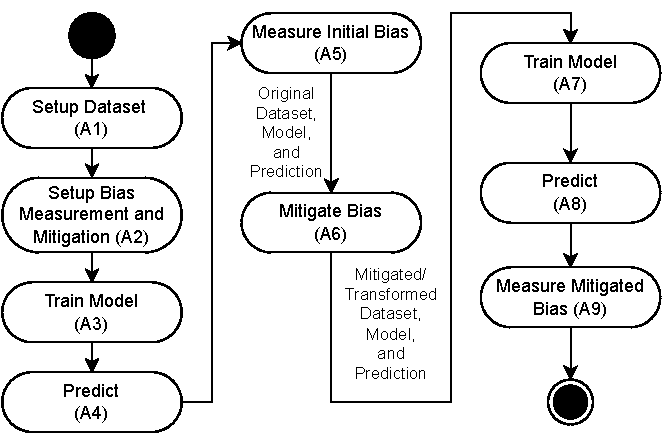
\includegraphics[width=\linewidth]{figures/workflow}
	\caption{The workflow of bias mitigation commonly performed using the toolkits in Section \ref{sec:toolkits}.}
	\label{fig:workflow}
\end{figure}

Our analysis found that, in general, all the toolkits perform the workflow presented in Figure \ref{fig:workflow}. Bias mitigation usually starts with setting up datasets (Action A1). In the action, users define the source of every dataset which is commonly a CSV file. They also profile each dataset to determine which attributes are the target/predicted attribute (including the favourable class in the attribute) and the sensitive attributes (including the privileged and unprivileged classes in the attributes).

In Action A2, users define the datasets and classifiers for model training. The training, validation, and test datasets are also set here, whether they are all come from different datasets or the same dataset but split with different ratios. They also select the bias metrics and mitigation algorithms that will be applied to datasets, models, and prediction. 

Users then train models in Action A3. The training can extend to validation for tuning hyper-parameters to obtain the best models. After that, users make prediction in Action A4 to measure the original accuracies of the models. The obtained accuracies will be compared against the accuracies post bias mitigation.
Users can skip the training and prediction (A3 and A4) if they only mitigate bias in the datasets, and the accuracies of prediction are not in concern.

Next, users measure the initial biases of the datasets, models, and prediction in Action A5. The scores of initial biases are used as benchmarks later on in the comparison against the scores of mitigated biases (A9). The results are compared

In the \textit{Mitigate Bias} action (A6), users apply bias mitigation algorithms to the original datasets, models, and predictions producing their bias-mitigated/transformed versions. In Action A7, the transformed datasets are then used to train new models (models created from bias-mitigated datasets). Using these models, together with models transformed from the original models in Action A6, users make new predictions (A8). 

Finally, after mitigated in Action A6, biases are measured again in Action A9. The mitigated biases are then compared to the original biases obtained in Action A5.  Users then analyse the results to find the best models with mitigated biases and accuracy that fit with their purposes. Results can be presented in numbers, tables, and charts to help users to examine the effects of the bias mitigation and choose the best models. 



\subsection{Design}
\label{sec:design}



\section{Evaluation}
\label{sec:evaluation}
In this research, we also evaluated the expressiveness, correctness, productivity, and execution time of FairML. In the expressiveness evaluation, we aimed to answer this question, 
``\textit{Can FairML express the use cases of bias mitigation in the real-world?}''. For that, we used the examples provided IBM Fairness AI 360 as the baseline to justify the expressiveness of FairML. 
the toolkit comes with a number of examples (Tables \ref{tab:expressiveness1} and \ref{tab:expressiveness2}) that demonstrate 
the usecases of the toolkit in the real-world context. 
Among 22 examples that comes in version 4.0, we only used 21 of them, 
since the one that we excluded only explains the use of a class dedicated to yield bias metric explanation in JSON format. We also count the numbers of bias metrics, de-biasing algorithms, classifiers, datasets, and measurement values are there in each example to reveal its complexity. 

We compared the bias metric values measured (measurement values) in the original examples with the values measured in the generated code to evaluate the correctness of FairML's generated code. Both should produce equal values or similar values, up to 10\% tolerance, when randomness is required.  

In the productivity evaluation, 
we compared the ratio of the written vs. generated code of FairML vs.
code in the examples. 
While this metric does not always guaranteed productivity in the end due many factors, 
the number of lines written by users is significantly reduced. In the measurement, \textit{markdown}, whitespace, and commented lines were not counted.

We also measured the execution time of FairML.First, we measured the \textit{generation time} -- the time that FairML takes to completely generate the target code. Second, we compared the time taken by the generated target code against the example code to to complete their operations (\textit{generated execution time} vs. \textit{original execution time}). The evaluation was performed on a machine with Windows 10 64-bit operating system, 11th Gen Intel(R) Core(TM) i9-11900H @ 2.50GHz 8-core processors, 32.0 GB RAM DDR4, OpenJDK Runtime Environment 18.9 (build 11.0.14.1+1), and Python 3.9.7.

\section{Results and Discussion}
\label{sec:result_and_discussion}
In this section, we present and discuss the results of our FairML evaluation.

\subsection{Expressiveness and Correctness}
\label{sec:expressiveness_and_correctness}
Based on our evaluation, FairML was able to reproduce all the scenarios in all the 21 examples in Tables \ref{tab:expressiveness1} and \ref{tab:expressiveness2}. In total, all the scenarios covered 8 unique datasets (Adult, German, Compas, Lawschool GPA, MEPSDataset19, MEPSDataset20, MEPSDataset21), 6 classifiers (Logistic Regression, Linear Regression, Linear SVR, Decision Tree, Kernel Ridge, Random Forest), 13 bias mitigation algorithms (Adversarial Debiasing, Callibrated Equalising Odds, Disparate Impact Remover, Exponentiated Gradient Reduction, Gerryfair, Learning Fair Representation, Reweighing, Meta Fair Classification, Optimized Preprocessing, Reject Option Classification, Prejudice Remover, Grid Search Reduction, Reweighing Meta), and 15 bias metrics (accuracy, balanced accuracy, mean a.k.a. statistical parity difference, disparate impact, equal opportunity difference, theil index, gamma disparity, average odds difference, mean absolute error, MDSS bias score, false positive rate, false negative rate, false discovery rate, error rate, mean absolute error). In addition, FairML also supports loading data from external CSV files. All of these allows users to express their bias mitigation strategies in different combinations of datasets, classifiers, de-biasing algorithms, and bias metrics.

Regarding correctness, the values that the generated code produced were dominantly equal to the measurement values in the examples. Some of them were different with tolerance less than $\pm$ 0.1 difference. From all $N$ measurement values in Tables \ref{tab:expressiveness1} and \ref{tab:expressiveness2}, equal values comprise $N1$ values, while the tolerated values cover only $N2$ values.  

%\newcolumntype{L}[1]{>{\raggedright\let\newline\\\arraybackslash\hspace{0pt}}m{#1}}
%\newcolumntype{C}[1]{>{\centering\let\newline\\\arraybackslash\hspace{0pt}}m{#1}}
%\newcolumntype{R}[1]{>{\raggedleft\let\newline\\\arraybackslash\hspace{0pt}}m{#1}}

\newcolumntype{L}[1]{>{\raggedright\arraybackslash}p{#1}}
\newcolumntype{C}[1]{>{\centering\arraybackslash}p{#1}}
\newcolumntype{R}[1]{>{\raggedleft\arraybackslash}p{#1}}


\begin{table*}[]
	\caption{Part I -- IBM AI Fairness 360 examples and the numbers of unique datasets, classifiers, de-biasing algorithms, bias metrics, and measurement values in each example.}
	\label{tab:expressiveness1}
	\begin{tabular}{ p{1em} L{10em} R{4em} R{8em} R{9em} R{12em} R{2.5em} }
		\hline
		\multicolumn{1}{c}{\textbf{Code}} &
		\multicolumn{1}{c}{\textbf{\begin{tabular}[c]{@{}c@{}}Example/File Name\\ (*.ipynb)\end{tabular}}} &
		\multicolumn{1}{c}{\textbf{Datasets}} &
		\multicolumn{1}{c}{\textbf{Classifiers}} &
		\multicolumn{1}{c}{\textbf{\begin{tabular}[c]{@{}c@{}}Debiasing\\ Algorithms\end{tabular}}} &
		\multicolumn{1}{c}{\textbf{\begin{tabular}[c]{@{}c@{}}Bias\\Metrics\end{tabular}}} &
		\multicolumn{1}{c}{\textbf{\begin{tabular}[c]{@{}c@{}}Mea-\\sure-\\ments\end{tabular}}} \\ \hline
		E01 &
		Demo Adversarial Debiasing &
		Adult &
		N/A &
		Adversarial debiasing &
		Accuracy, Balanced accuracy, Disparate impact, Average odds, Statistical parity, Equal opportunity, Theil index &
		28 \\
		E02 &
		Demo Callibrated Eq Odd Postprocessing &
		Adult, German, Compas &
		Logistic regression &
		Calibrated eq odds postprocessing &
		Mean difference, False positive rate, False negative rate, Balanced accuracy, Equal opportunity &
		13 \\
		E03 &
		Demo Disparate Impact Remover &
		Adult &
		Logistic regression &
		Disparate impact remover &
		Disparate impact &
		11 \\
		E04 &
		Demo Exponentiated Gradient Reduction &
		Adult &
		Logistic regression &
		Exponentiated gradient reduction &
		Accuracy, Mean difference, Average odds &
		8 \\
		E05 &
		Demo Gerryfair &
		Adult &
		Linear Regression, Linear SVR, Decision Tree, Kernel Ridge &
		Gerryfair &
		Gamma disparity &
		31 \\
		E06 &
		Demo LFR &
		Adult &
		Logistic regression &
		Learning fair representation &
		Balanced accuracy, Mean difference, Disparate impact &
		5 \\
		E07 &
		Demo Lime &
		Adult &
		Logistic regression, Random forest &
		Reweighing &
		Accuracy, Balanced accuracy, Disparate impact, Average odds &
		6 \\
		E08 &
		Demo MDSS Classifier Metric &
		Compas &
		Logistic regression &
		Meta fair classifier &
		Mean difference, MDSS bias score &
		7 \\
		E09 &
		Demo Meta Classifier &
		Adult &
		N/A &
		Meta fair classifier &
		Accuracy, Balanced accuracy, Disparate impact, False discovery rate &
		13 \\
		E10 &
		Demo Optim Data Preproc &
		Adult, German, Compas &
		Logistic regression &
		Optimized preprocessing &
		Balanced accuracy, Disparate impact, Average odds, Statistical parity &
		9 \\
		E11 &
		Demo Optim Preproc Adult &
		Adult &
		N/A &
		Optimized preprocessing &
		Mean difference &
		2 \\
	 	\hline
	\end{tabular}
\end{table*}

\begin{table*}[]
	\caption{Part II -- IBM AI Fairness 360 examples and the numbers of unique datasets, classifiers, de-biasing algorithms, bias metrics, and measurement values in each example.}
	\label{tab:expressiveness2}
	\begin{tabular}{ p{1em} L{10em} R{4em} R{8em} R{9em} R{12em} R{2.5em} }
		\hline
		\multicolumn{1}{c}{\textbf{Code}} &
		\multicolumn{1}{c}{\textbf{\begin{tabular}[c]{@{}c@{}}Example/File Name\\ (*.ipynb)\end{tabular}}} &
		\multicolumn{1}{c}{\textbf{Datasets}} &
		\multicolumn{1}{c}{\textbf{Classifiers}} &
		\multicolumn{1}{c}{\textbf{\begin{tabular}[c]{@{}c@{}}Debiasing\\ Algorithms\end{tabular}}} &
		\multicolumn{1}{c}{\textbf{\begin{tabular}[c]{@{}c@{}}Bias\\Metrics\end{tabular}}} &
		\multicolumn{1}{c}{\textbf{\begin{tabular}[c]{@{}c@{}}Mea-\\sure-\\ments\end{tabular}}} \\ \hline
		E12 &
		Demo Reject Option Classification &
		Adult, German, Compas &
		Logistic Regression &
		Reject option classification &
		Balanced accuracy, Disparate impact, Average odds, Statistical parity, Equal opportunity, Theil index &
		26 \\
		E13 &
		Demo Reweighing Preproc &
		Adult, German, Compas &
		Logistic Regression &
		Reweighing &
		Balanced accuracy, Disparate impact, Average odds,. Statistical parity, Equal opportunity, Theil index &
		16 \\
		E14 &
		Demo Short Gerryfair Test &
		Adult &
		Linear Regression, Linear SVR, Decision Tree, Kernel Ridge &
		Gerryfair &
		Gamma disparity &
		13 \\
		E15 &
		Tutorial Credit Scoring &
		German &
		N/A &
		Reweighing &
		Mean difference &
		2 \\
		E16 &
		Tutorial Medical Expenditure &
		MEPS-Dataset19, MEPSDataset20, MEPSDataset21 &
		Random Forest, Logistic Regression &
		Reweighing, Prejudice remover &
		Balanced accuracy, Disparate impact, Average odds, Statistical parity, Equal opportunity, Theil index &
		90 \\
		E17 &
		Demo Exponentiated Gradient Reduction Sklearn &
		Adult &
		Logistic Regression &
		Grid search reduction &
		\begin{tabular}[c]{@{}r@{}}Average odds\\ Accuracy\end{tabular} &
		7 \\
		E18 &
		Demo Grid Search Reduction Classification Sklearn &
		Adult &
		Logistic Regression &
		Grid search reduction &
		Average odds, Accuracy &
		4 \\
		E19 &
		Demo Grid Search Reduction Regression Sklearn &
		Lawschool GPA &
		Linear Regression &
		Grid search reduction &
		Mean absolute error &
		7 \\
		E20 &
		Demo MDSS Classifier Metric Sklearn &
		Compas &
		Logistic Regression &
		N/A &
		MDSS bias score &
		4 \\
		E21 &
		Demo New Features &
		Adult &
		Logistic Regression &
		Reweighing meta, Adversarial debiasing, Callibrated equalized odd &
		Disparate impact, Average odds, Mean difference, Accuracy &
		6 \\ \hline
	\end{tabular}
\end{table*}


\subsection{Productivity}
\label{sec:productivity}

Table \ref{tab:loc} shows a comparison on the numbers of lines of code (LoC) between the original examples, FairML models, and generated code. It shows that \textsf{Model LoC}/\textsf{Original LoC} are equal or less than 1, indicating that users would write less code to produce the same results as in the examples (see Section \ref{sec:expressiveness_and_correctness} for correctness). Moreover, the efficiency also gets higher as the number of original LoC increases as can been seen at the examples \textsf{E15} and \textsf{E16}, where LoC goes up from 30 to 356, that the efficiency is also increased -- with users only need to write from 83\% to 25\% of the LoC in their respective original examples.

We do expect that FairML generates more LoC than the original examples as they contain features that are no included in the original examples, such as (1) the code for explaining the classifiers, bias mitigation algorithms, and bias metrics being used, as well as (2) the code for displaying summary tables and charts. 

%We do admit that there are also generated lines of code that are not always necessary for every scenario but always exist in the code -- this also increases the number of generated LoC.For example,   

\begin{table*}[]
	\caption{Lines of code of the original examples (Ori LoC), FairML models (Model LoC), and generated code (Gen LoC).}
	\label{tab:loc}
	\begin{tabular}{clrrrrrr}
		\hline
		\multicolumn{1}{c}{\textbf{Code}} &
		\multicolumn{1}{c}{\textbf{\begin{tabular}[c]{@{}c@{}}Example/File Name \\ (*.ipynb)\end{tabular}}} &
		\multicolumn{1}{c}{\textbf{\begin{tabular}[c]{@{}c@{}}Ori\\ LoC\end{tabular}}} &
		\multicolumn{1}{c}{\textbf{\begin{tabular}[c]{@{}c@{}}Model\\ LoC\end{tabular}}} &
		\multicolumn{1}{c}{\textbf{\begin{tabular}[c]{@{}c@{}}Gen\\ LoC\end{tabular}}} &
		\multicolumn{1}{c}{\textbf{\begin{tabular}[c]{@{}c@{}}Model  LoC/\\ Ori  LoC\end{tabular}}} &
		\multicolumn{1}{c}{\textbf{\begin{tabular}[c]{@{}c@{}}Gen LoC/\\ Model LoC\end{tabular}}} &
		\multicolumn{1}{c}{\textbf{\begin{tabular}[c]{@{}c@{}}Gen LoC/\\ Ori LoC\end{tabular}}} \\ \hline
		E01 & Demo Adversarial Debiasing                        & 133 &    &     &      &      &      \\
		E02 & Demo Callibrated Eqodd Postprocessing             & 257 &    &     &      &      &      \\
		E03 & Demo Disparate Impact Remover                     & 50  & 50 & 367 & 1.00 & 7.34 & 7.34 \\
		E04 & Demo Exponentiated Gradient Reduction             & 93  & 33 & 110 & 0.35 & 3.33 & 1.18 \\
		E05 & Demo Gerryfair                                    & 90  &    &     &      &      &      \\
		E06 & Demo LFR                                          & 103 &    &     &      &      &      \\
		E07 & Demo   Lime                                       & 238 &    &     &      &      &      \\
		E08 & Demo MDSS Classifier Metric                       & 130 &    &     &      &      &      \\
		E09 & Demo Meta Classifier                              & 95  & 67 & 345 & 0.71 & 5.15 & 3.63 \\
		E10 & Demo Optim Data Preproc                           & 233 &    &     &      &      &      \\
		E11 & Demo Optim Preproc Adult                          & 35  & 30 & 85  & 0.86 & 2.83 & 2.43 \\
		E12 & Demo Reject Option Classification                 & 143 &    &     &      &      &      \\
		E13 & Demo Reweighing Preproc                           & 212 & 59 & 125 & 0.28 & 2.12 & 0.59 \\
		E14 & Demo Short Gerryfair Test                         & 52  & 50 & 176 & 0.96 & 3.52 & 3.38 \\
		E15 & Tutorial Credit Scoring                           & 30  & 25 & 84  & 0.83 & 3.36 & 2.80 \\
		E16 & Tutorial Medical Expenditure                      & 356 & 90 & 554 & 0.25 & 6.16 & 1.56 \\
		E17 & Demo Exponentiated Gradient Reduction Sklearn     & 54  &    &     &      &      &      \\
		E18 & Demo Grid Search Reduction Classification Sklearn & 52  &    &     &      &      &      \\
		E19 & Demo Grid Search Reduction Regression Sklearn     & 64  &    &     &      &      &      \\
		E20 & Demo MDSS Classifier Metric Sklearn               & 66  &    &     &      &      &      \\
		E21 & Demo New Features                                 & 82  &    &     &      &      &      \\ \hline
	\end{tabular}
\end{table*}


\subsection{Execution Time}
\label{sec:execution_time}

Table \ref{tab:time} shows the duration -- generation time -- taken by FairML to produce generated code, 
and the performance of the generated code on execution time against the original examples (in seconds). 
On the generation time, 
FairML is able to generate every generated-code version of the original examples in less that 0.2 seconds, 
and it can achieve the rate 2,798 lines/second based on the example E16 
(554 lines/0.198 seconds, Tables \ref{tab:loc} and \ref{tab:time}). 

In general, the execution time of the generated code takes more time than the original examples. 
We do anticipate this as the generated-code versions have more features, having more lines of code,
as stated in Section \ref{sec:productivity}. 

 

\begin{table*}[]
	\caption{The generation time of FairML and execution time of the original examples and generated code (seconds).}
	\label{tab:time}
	\begin{tabular}{clrrrr}
		\hline
		\textbf{Code} &
		\multicolumn{1}{c}{\textbf{\begin{tabular}[c]{@{}c@{}}Example/File Name \\ (*.ipynb)\end{tabular}}} &
		\multicolumn{1}{c}{\textbf{\begin{tabular}[c]{@{}c@{}}Generation\\ Time\end{tabular}}} &
		\multicolumn{1}{c}{\textbf{\begin{tabular}[c]{@{}c@{}}Original\\ Exec Time\end{tabular}}} &
		\multicolumn{1}{c}{\textbf{\begin{tabular}[c]{@{}c@{}}Generated\\ Exec Time\end{tabular}}} &
		\multicolumn{1}{c}{\textbf{\begin{tabular}[c]{@{}c@{}}Gen/Ori\\ Exec Time\end{tabular}}} \\ \hline
		E01 & Demo Adversarial Debiasing                        &       &        &        &      \\
		E02 & Demo Callibrated Eqodd Postprocessing             &       &        &        &      \\
		E03 & Demo Disparate Impact Remover                     & 0.186 & 20.991 & 20.23  & 0.96 \\
		E04 & Demo Exponentiated Gradient Reduction             & 0.166 & 29.927 & 30.211 & 1.01 \\
		E05 & Demo Gerryfair                                    &       &        &        &      \\
		E06 & Demo LFR                                          &       &        &        &      \\
		E07 & Demo   Lime                                       &       &        &        &      \\
		E08 & Demo MDSS Classifier Metric                       &       &        &        &      \\
		E09 & Demo Meta Classifier                              & 0.192 & 12.989 & 14.67  & 1.13 \\
		E10 & Demo Optim Data Preproc                           &       &        &        &      \\
		E11 & Demo Optim Preproc Adult                          & 0.154 & 8.044  & 15.52  & 1.93 \\
		E12 & Demo Reject Option Classification                 &       &        &        &      \\
		E13 & Demo Reweighing Preproc                           & 0.158 & 1.461  & 4.633  & 3.17 \\
		E14 & Demo Short Gerryfair Test                         & 0.164 & 3.389  & 3.875  & 1.14 \\
		E15 & Tutorial Credit Scoring                           & 0.162 & 0.017  & 0.078  & 4.59 \\
		E16 & Tutorial Medical Expenditure                      & 0.198 & 34.897 & 54.248 & 1.55 \\
		E17 & Demo Exponentiated Gradient Reduction Sklearn     &       &        &        &      \\
		E18 & Demo Grid Search Reduction Classification Sklearn &       &        &        &      \\
		E19 & Demo Grid Search Reduction Regression Sklearn     &       &        &        &      \\
		E20 & Demo MDSS Classifier Metric Sklearn               &       &        &        &      \\
		E21 & Demo New Features                                 &       &        &        &      \\ \hline
	\end{tabular}
\end{table*}
'
\section{Lessons Learned}
\label{sec:lessons_learned}



%\section{Related Work}
%\label{sec:related_work}


\section{Conclusions and Future Work}
\label{sec:conclusions_and_future_work}
In this paper, we have presented FairML, a toolkit that implements a model-based approach to automate bias mitigation. Using FairML, users can generate bias mitigation code with writing less lines in YAML compared to writing the code in Python, a general programming language.
In terms of correctness, the generated code produces the same bias metric values as measured in the original examples.

As the development of FairML is still in the early stage, 
there is much room for improvement as future work. For examples, the number of lines of code generated by FairML can still be further reduced by merging repeatable lines into functions and removing unnecessary code determined by firstly performing static analysis. 
As the knock-on effect, the removal of unnecessary code can optimise the execution time of the generated code. 

%% The Appendices part is started with the command \appendix;
%% appendix sections are then done as normal sections
\appendix

\section{List of Examples}
\label{sec:list_of_examples}




\section{List of Constructs}
\label{sec:list_of_constructs}



\begin{enumerate}
	\item Dataset.
	\item Label or Predicted/Target Attribute.
	\item Favourable Class/Group.
	\item Protected/Sensitive Attribute.
	\item Privileged Group/Class.
	\item Unprivileged Group/Class.
	\item Bias Metric.
	\item Bias Mitigation.
	\item Classifier.
	\item Model.
	\item Prediction.
	\item Bias Mitigation Algorithm.
	\item Training.
	\item Test.
	\item Validation.
	\item Accuracy.
	\item Bias.
	\item Parameters.
\end{enumerate}

  \bibliographystyle{ACM-Reference-Format} 
\bibliography{references}

\end{document}
\endinput
%%
%% End of file `sample-sigconf.tex'.
